\documentclass[12pt,a4paper]{article}

\usepackage[a4paper,text={16.5cm,25.2cm},centering]{geometry}
\usepackage{lmodern}
\usepackage{amssymb,amsmath}
\usepackage{bm}
\usepackage{graphicx}
\usepackage{microtype}
\usepackage{hyperref}
\setlength{\parindent}{0pt}
\setlength{\parskip}{1.2ex}

\hypersetup
       {   pdfauthor = { Rodrigo A Morales M },
           pdftitle={ 714, computational econ, PS01 },
           colorlinks=TRUE,
           linkcolor=black,
           citecolor=blue,
           urlcolor=blue
       }

\title{ 714, computational econ, PS01 }

\author{ Rodrigo A Morales M }

\date{ 2nd December 2019 }

\usepackage{upquote}
\usepackage{listings}
\usepackage{xcolor}
\lstset{
    basicstyle=\ttfamily\footnotesize,
    upquote=true,
    breaklines=true,
    breakindent=0pt,
    keepspaces=true,
    showspaces=false,
    columns=fullflexible,
    showtabs=false,
    showstringspaces=false,
    escapeinside={(*@}{@*)},
    extendedchars=true,
}
\newcommand{\HLJLt}[1]{#1}
\newcommand{\HLJLw}[1]{#1}
\newcommand{\HLJLe}[1]{#1}
\newcommand{\HLJLeB}[1]{#1}
\newcommand{\HLJLo}[1]{#1}
\newcommand{\HLJLk}[1]{\textcolor[RGB]{148,91,176}{\textbf{#1}}}
\newcommand{\HLJLkc}[1]{\textcolor[RGB]{59,151,46}{\textit{#1}}}
\newcommand{\HLJLkd}[1]{\textcolor[RGB]{214,102,97}{\textit{#1}}}
\newcommand{\HLJLkn}[1]{\textcolor[RGB]{148,91,176}{\textbf{#1}}}
\newcommand{\HLJLkp}[1]{\textcolor[RGB]{148,91,176}{\textbf{#1}}}
\newcommand{\HLJLkr}[1]{\textcolor[RGB]{148,91,176}{\textbf{#1}}}
\newcommand{\HLJLkt}[1]{\textcolor[RGB]{148,91,176}{\textbf{#1}}}
\newcommand{\HLJLn}[1]{#1}
\newcommand{\HLJLna}[1]{#1}
\newcommand{\HLJLnb}[1]{#1}
\newcommand{\HLJLnbp}[1]{#1}
\newcommand{\HLJLnc}[1]{#1}
\newcommand{\HLJLncB}[1]{#1}
\newcommand{\HLJLnd}[1]{\textcolor[RGB]{214,102,97}{#1}}
\newcommand{\HLJLne}[1]{#1}
\newcommand{\HLJLneB}[1]{#1}
\newcommand{\HLJLnf}[1]{\textcolor[RGB]{66,102,213}{#1}}
\newcommand{\HLJLnfm}[1]{\textcolor[RGB]{66,102,213}{#1}}
\newcommand{\HLJLnp}[1]{#1}
\newcommand{\HLJLnl}[1]{#1}
\newcommand{\HLJLnn}[1]{#1}
\newcommand{\HLJLno}[1]{#1}
\newcommand{\HLJLnt}[1]{#1}
\newcommand{\HLJLnv}[1]{#1}
\newcommand{\HLJLnvc}[1]{#1}
\newcommand{\HLJLnvg}[1]{#1}
\newcommand{\HLJLnvi}[1]{#1}
\newcommand{\HLJLnvm}[1]{#1}
\newcommand{\HLJLl}[1]{#1}
\newcommand{\HLJLld}[1]{\textcolor[RGB]{148,91,176}{\textit{#1}}}
\newcommand{\HLJLs}[1]{\textcolor[RGB]{201,61,57}{#1}}
\newcommand{\HLJLsa}[1]{\textcolor[RGB]{201,61,57}{#1}}
\newcommand{\HLJLsb}[1]{\textcolor[RGB]{201,61,57}{#1}}
\newcommand{\HLJLsc}[1]{\textcolor[RGB]{201,61,57}{#1}}
\newcommand{\HLJLsd}[1]{\textcolor[RGB]{201,61,57}{#1}}
\newcommand{\HLJLsdB}[1]{\textcolor[RGB]{201,61,57}{#1}}
\newcommand{\HLJLsdC}[1]{\textcolor[RGB]{201,61,57}{#1}}
\newcommand{\HLJLse}[1]{\textcolor[RGB]{59,151,46}{#1}}
\newcommand{\HLJLsh}[1]{\textcolor[RGB]{201,61,57}{#1}}
\newcommand{\HLJLsi}[1]{#1}
\newcommand{\HLJLso}[1]{\textcolor[RGB]{201,61,57}{#1}}
\newcommand{\HLJLsr}[1]{\textcolor[RGB]{201,61,57}{#1}}
\newcommand{\HLJLss}[1]{\textcolor[RGB]{201,61,57}{#1}}
\newcommand{\HLJLssB}[1]{\textcolor[RGB]{201,61,57}{#1}}
\newcommand{\HLJLnB}[1]{\textcolor[RGB]{59,151,46}{#1}}
\newcommand{\HLJLnbB}[1]{\textcolor[RGB]{59,151,46}{#1}}
\newcommand{\HLJLnfB}[1]{\textcolor[RGB]{59,151,46}{#1}}
\newcommand{\HLJLnh}[1]{\textcolor[RGB]{59,151,46}{#1}}
\newcommand{\HLJLni}[1]{\textcolor[RGB]{59,151,46}{#1}}
\newcommand{\HLJLnil}[1]{\textcolor[RGB]{59,151,46}{#1}}
\newcommand{\HLJLnoB}[1]{\textcolor[RGB]{59,151,46}{#1}}
\newcommand{\HLJLoB}[1]{\textcolor[RGB]{102,102,102}{\textbf{#1}}}
\newcommand{\HLJLow}[1]{\textcolor[RGB]{102,102,102}{\textbf{#1}}}
\newcommand{\HLJLp}[1]{#1}
\newcommand{\HLJLc}[1]{\textcolor[RGB]{153,153,119}{\textit{#1}}}
\newcommand{\HLJLch}[1]{\textcolor[RGB]{153,153,119}{\textit{#1}}}
\newcommand{\HLJLcm}[1]{\textcolor[RGB]{153,153,119}{\textit{#1}}}
\newcommand{\HLJLcp}[1]{\textcolor[RGB]{153,153,119}{\textit{#1}}}
\newcommand{\HLJLcpB}[1]{\textcolor[RGB]{153,153,119}{\textit{#1}}}
\newcommand{\HLJLcs}[1]{\textcolor[RGB]{153,153,119}{\textit{#1}}}
\newcommand{\HLJLcsB}[1]{\textcolor[RGB]{153,153,119}{\textit{#1}}}
\newcommand{\HLJLg}[1]{#1}
\newcommand{\HLJLgd}[1]{#1}
\newcommand{\HLJLge}[1]{#1}
\newcommand{\HLJLgeB}[1]{#1}
\newcommand{\HLJLgh}[1]{#1}
\newcommand{\HLJLgi}[1]{#1}
\newcommand{\HLJLgo}[1]{#1}
\newcommand{\HLJLgp}[1]{#1}
\newcommand{\HLJLgs}[1]{#1}
\newcommand{\HLJLgsB}[1]{#1}
\newcommand{\HLJLgt}[1]{#1}


\begin{document}

\maketitle

\section{UPENN}
\subsection{Econ, 714}
\#\#\#Problem Set 01

\subsubsection{Intro}
This is just a test for the problem set, when $\beta =2.1$: $\alpha = 0.4$


\begin{lstlisting}
Packages are retrieved...
\end{lstlisting}


\begin{lstlisting}
Packages gotten alright, getting modules...
\end{lstlisting}


\begin{lstlisting}
modules loaded ok
\end{lstlisting}


An inline image 2 is: \begin{figure}
\centering
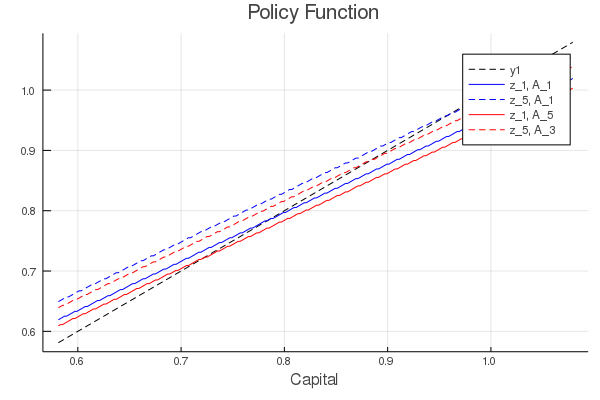
\includegraphics{Plots/000_PolicyFunction_a_fixed_grid_20191129.png}
\caption{Plot example01}
\end{figure}



\begin{lstlisting}
(*@\HLJLcs{{\#}}@*) (*@\HLJLcs{------------------------------------------------------------------------------}@*)
(*@\HLJLcs{{\#}}@*) (*@\HLJLcs{1.}@*) (*@\HLJLcs{Set}@*) (*@\HLJLcs{Parameters}@*) (*@\HLJLcs{(building}@*) (*@\HLJLcs{structure)}@*)
(*@\HLJLn{econ{\_}params}@*) (*@\HLJLoB{=}@*) (*@\HLJLnd{@with{\_}kw}@*) (*@\HLJLp{(}@*)
                (*@\HLJLn{\ensuremath{\alpha}}@*) (*@\HLJLoB{=}@*) (*@\HLJLnfB{0.33}@*)(*@\HLJLp{,}@*)   (*@\HLJLcs{{\#}}@*) (*@\HLJLcs{kaptl}@*) (*@\HLJLcs{share}@*)
                (*@\HLJLn{\ensuremath{\beta}}@*) (*@\HLJLoB{=}@*) (*@\HLJLnfB{0.96}@*)(*@\HLJLp{,}@*)   (*@\HLJLcs{{\#}}@*) (*@\HLJLcs{time}@*) (*@\HLJLcs{discount}@*)
                (*@\HLJLn{\ensuremath{\delta}}@*) (*@\HLJLoB{=}@*) (*@\HLJLnfB{0.1}@*)(*@\HLJLp{,}@*)    (*@\HLJLcs{{\#}}@*) (*@\HLJLcs{deprectn}@*)
                (*@\HLJLn{\ensuremath{\theta}}@*) (*@\HLJLoB{=}@*) (*@\HLJLnfB{0.5}@*)(*@\HLJLp{,}@*)    (*@\HLJLcs{{\#}}@*) (*@\HLJLcs{elast}@*) (*@\HLJLcs{subs}@*) (*@\HLJLcs{tween}@*) (*@\HLJLcs{goods}@*)
                (*@\HLJLn{maxiter}@*) (*@\HLJLoB{=}@*) (*@\HLJLni{1000}@*)(*@\HLJLp{,}@*)
                (*@\HLJLcs{{\#}}@*) (*@\HLJLcs{Stochasticity}@*)
                (*@\HLJLn{vGridZ}@*)    (*@\HLJLoB{=}@*) (*@\HLJLp{[}@*)(*@\HLJLoB{-}@*)(*@\HLJLnfB{0.0673}@*)(*@\HLJLp{,}@*) (*@\HLJLoB{-}@*)(*@\HLJLnfB{0.0336}@*)(*@\HLJLp{,}@*)  (*@\HLJLni{0}@*)(*@\HLJLp{,}@*)      (*@\HLJLnfB{0.0336}@*)(*@\HLJLp{,}@*) (*@\HLJLnfB{0.0673}@*)(*@\HLJLp{],}@*)
                (*@\HLJLn{mTranstnZ}@*) (*@\HLJLoB{=}@*) (*@\HLJLp{[}@*) (*@\HLJLnfB{0.9727}@*)  (*@\HLJLnfB{0.0273}@*)    (*@\HLJLni{0}@*)       (*@\HLJLni{0}@*)       (*@\HLJLni{0}@*)(*@\HLJLp{;}@*)
                              (*@\HLJLnfB{0.0041}@*)  (*@\HLJLnfB{0.9806}@*)    (*@\HLJLnfB{0.0153}@*)  (*@\HLJLni{0}@*)       (*@\HLJLni{0}@*)(*@\HLJLp{;}@*)
                              (*@\HLJLni{0}@*)       (*@\HLJLnfB{0.0082}@*)    (*@\HLJLnfB{0.9836}@*)  (*@\HLJLnfB{0.0082}@*)  (*@\HLJLni{0}@*)(*@\HLJLp{;}@*)
                              (*@\HLJLni{0}@*)       (*@\HLJLni{0}@*)         (*@\HLJLnfB{0.0153}@*)  (*@\HLJLnfB{0.9806}@*)  (*@\HLJLnfB{0.0041}@*)(*@\HLJLp{;}@*)
                              (*@\HLJLni{0}@*)       (*@\HLJLni{0}@*)         (*@\HLJLni{0}@*)       (*@\HLJLnfB{0.0273}@*)  (*@\HLJLnfB{0.9727}@*)(*@\HLJLp{],}@*)
                (*@\HLJLcs{{\#}}@*) (*@\HLJLcs{production}@*) (*@\HLJLcs{func.}@*) (*@\HLJLcs{2}@*)
                (*@\HLJLn{vGridA}@*)    (*@\HLJLoB{=}@*) (*@\HLJLp{[}@*)  (*@\HLJLnfB{0.9}@*)(*@\HLJLp{,}@*)  (*@\HLJLni{1}@*)(*@\HLJLp{,}@*)    (*@\HLJLnfB{1.1}@*)(*@\HLJLp{],}@*)
                (*@\HLJLn{mTranstnA}@*) (*@\HLJLoB{=}@*) (*@\HLJLp{[}@*)  (*@\HLJLnfB{0.9}@*)   (*@\HLJLnfB{0.1}@*)   (*@\HLJLni{0}@*)(*@\HLJLp{;}@*)
                               (*@\HLJLnfB{0.05}@*)  (*@\HLJLnfB{0.9}@*)   (*@\HLJLnfB{0.05}@*)(*@\HLJLp{;}@*)
                               (*@\HLJLni{0}@*)     (*@\HLJLnfB{0.1}@*)   (*@\HLJLnfB{0.9}@*)(*@\HLJLp{],}@*)
                (*@\HLJLn{mTranstnZA}@*) (*@\HLJLoB{=}@*) (*@\HLJLnf{kron}@*)(*@\HLJLp{(}@*)(*@\HLJLn{mTranstnZ}@*)(*@\HLJLp{,}@*)(*@\HLJLn{mTranstnA}@*)(*@\HLJLp{)}@*)
        (*@\HLJLp{)}@*)
(*@\HLJLcs{{\#}}@*) (*@\HLJLcs{once}@*) (*@\HLJLcs{structure}@*) (*@\HLJLcs{is}@*) (*@\HLJLcs{built,}@*) (*@\HLJLcs{call}@*) (*@\HLJLcs{it}@*) (*@\HLJLcs{to}@*) (*@\HLJLcs{use}@*) (*@\HLJLcs{in}@*) (*@\HLJLcs{VFIs}@*) (*@\HLJLcs{(fixed}@*) (*@\HLJLcs{grid,}@*) (*@\HLJLcs{etc...)}@*)
(*@\HLJLn{econparams}@*) (*@\HLJLoB{=}@*) (*@\HLJLnf{econ{\_}params}@*)(*@\HLJLp{()}@*)  (*@\HLJLcs{{\#}call}@*) (*@\HLJLcs{function}@*) (*@\HLJLcs{and}@*) (*@\HLJLcs{get}@*) (*@\HLJLcs{the}@*) (*@\HLJLcs{relevant}@*) (*@\HLJLcs{parameters}@*) (*@\HLJLcs{4}@*) (*@\HLJLcs{ss}@*)
(*@\HLJLn{dosave}@*) (*@\HLJLoB{=}@*) (*@\HLJLni{0}@*)
(*@\HLJLn{doload}@*) (*@\HLJLoB{=}@*) (*@\HLJLni{0}@*)
(*@\HLJLnd{@unpack}@*) (*@\HLJLn{\ensuremath{\alpha}}@*)(*@\HLJLp{,}@*) (*@\HLJLn{\ensuremath{\beta}}@*)(*@\HLJLp{,}@*) (*@\HLJLn{\ensuremath{\delta}}@*)(*@\HLJLp{,}@*) (*@\HLJLn{\ensuremath{\theta}}@*)(*@\HLJLp{,}@*) (*@\HLJLn{vGridZ}@*)(*@\HLJLp{,}@*) (*@\HLJLn{vGridA}@*)  (*@\HLJLoB{=}@*) (*@\HLJLn{econparams}@*)
(*@\HLJLcs{{\#}}@*) (*@\HLJLcs{------------------------------------------------------------------------------}@*)
(*@\HLJLcs{{\#}}@*) (*@\HLJLcs{2.}@*) (*@\HLJLcs{Steady}@*) (*@\HLJLcs{State,}@*) (*@\HLJLcs{solve}@*) (*@\HLJLcs{for:}@*)
(*@\HLJLn{xinit}@*) (*@\HLJLoB{=}@*)  (*@\HLJLp{[}@*)(*@\HLJLnfB{0.5}@*)(*@\HLJLp{,}@*) (*@\HLJLnfB{0.5}@*)(*@\HLJLp{,}@*) (*@\HLJLni{1}@*)(*@\HLJLp{]}@*) (*@\HLJLcs{{\#}[0.2,}@*) (*@\HLJLcs{0.2,}@*) (*@\HLJLcs{0.8]}@*) (*@\HLJLcs{{\#}[0.5,}@*) (*@\HLJLcs{0.5,}@*) (*@\HLJLcs{1]}@*) (*@\HLJLcs{{\#}initial}@*) (*@\HLJLcs{value}@*) (*@\HLJLcs{to}@*) (*@\HLJLcs{find}@*) (*@\HLJLcs{ss}@*)
(*@\HLJLn{sssol}@*) (*@\HLJLoB{=}@*)  (*@\HLJLn{ss{\_}deterministic}@*)(*@\HLJLoB{.}@*)(*@\HLJLnf{ss{\_}solver}@*)(*@\HLJLp{(}@*)(*@\HLJLn{xinit}@*)(*@\HLJLp{,}@*) (*@\HLJLn{\ensuremath{\alpha}}@*)(*@\HLJLp{,}@*) (*@\HLJLn{\ensuremath{\beta}}@*)(*@\HLJLp{,}@*) (*@\HLJLn{\ensuremath{\delta}}@*)(*@\HLJLp{,}@*) (*@\HLJLn{\ensuremath{\theta}}@*) (*@\HLJLp{)}@*)
(*@\HLJLn{l1ss}@*)  (*@\HLJLoB{=}@*)  (*@\HLJLn{sssol}@*)(*@\HLJLoB{.}@*)(*@\HLJLn{zero}@*)(*@\HLJLp{[}@*)(*@\HLJLni{1}@*)(*@\HLJLp{]}@*)
(*@\HLJLn{l2ss}@*)  (*@\HLJLoB{=}@*)  (*@\HLJLn{sssol}@*)(*@\HLJLoB{.}@*)(*@\HLJLn{zero}@*)(*@\HLJLp{[}@*)(*@\HLJLni{2}@*)(*@\HLJLp{]}@*)
(*@\HLJLn{kss}@*)   (*@\HLJLoB{=}@*)  (*@\HLJLn{sssol}@*)(*@\HLJLoB{.}@*)(*@\HLJLn{zero}@*)(*@\HLJLp{[}@*)(*@\HLJLni{3}@*)(*@\HLJLp{]}@*)

(*@\HLJLcs{{\#}}@*) (*@\HLJLcs{the}@*) (*@\HLJLcs{rest}@*) (*@\HLJLcs{are}@*) (*@\HLJLcs{determined}@*) (*@\HLJLcs{by}@*) (*@\HLJLcs{k,l1,l2}@*)
(*@\HLJLn{lss}@*)   (*@\HLJLoB{=}@*)  (*@\HLJLn{l1ss}@*) (*@\HLJLoB{+}@*) (*@\HLJLn{l2ss}@*)
(*@\HLJLn{c1ss}@*)  (*@\HLJLoB{=}@*)  (*@\HLJLn{kss}@*)(*@\HLJLoB{{\textasciicircum}}@*)(*@\HLJLp{(}@*)(*@\HLJLn{\ensuremath{\alpha}}@*)(*@\HLJLp{)}@*) (*@\HLJLoB{*}@*) (*@\HLJLn{l1ss}@*)(*@\HLJLoB{{\textasciicircum}}@*)(*@\HLJLp{(}@*)(*@\HLJLni{1}@*)(*@\HLJLoB{-}@*)(*@\HLJLn{\ensuremath{\alpha}}@*)(*@\HLJLp{)}@*) (*@\HLJLoB{-}@*) (*@\HLJLn{\ensuremath{\delta}}@*) (*@\HLJLoB{*}@*) (*@\HLJLn{kss}@*)
(*@\HLJLn{c2ss}@*)  (*@\HLJLoB{=}@*)  (*@\HLJLn{l2ss}@*)

(*@\HLJLnf{println}@*)(*@\HLJLp{(}@*)(*@\HLJLs{"{}}@*) (*@\HLJLs{Steady}@*) (*@\HLJLs{state}@*) (*@\HLJLs{"{}}@*)(*@\HLJLp{)}@*)
\end{lstlisting}

\begin{lstlisting}
Steady state
\end{lstlisting}


\begin{lstlisting}
(*@\HLJLnf{println}@*)(*@\HLJLp{(}@*)(*@\HLJLs{"{}K{\_}ss}@*) (*@\HLJLs{=}@*) (*@\HLJLs{"{}}@*)(*@\HLJLp{,}@*) (*@\HLJLn{kss}@*)(*@\HLJLp{,}@*) (*@\HLJLs{"{}}@*)  (*@\HLJLs{L{\_}ss}@*) (*@\HLJLs{=}@*) (*@\HLJLs{"{}}@*)(*@\HLJLp{,}@*) (*@\HLJLn{lss}@*)(*@\HLJLp{,}@*) (*@\HLJLs{"{}}@*)  (*@\HLJLs{C1{\_}ss}@*) (*@\HLJLs{=}@*) (*@\HLJLs{"{}}@*)(*@\HLJLp{,}@*) (*@\HLJLn{c1ss}@*)(*@\HLJLp{,}@*) (*@\HLJLs{"{}}@*) (*@\HLJLs{C2{\_}ss}@*) (*@\HLJLs{=}@*) (*@\HLJLs{"{}}@*)(*@\HLJLp{,}@*) (*@\HLJLn{c2ss}@*)(*@\HLJLp{)}@*)
\end{lstlisting}

\begin{lstlisting}
K_ss = 0.8301903102383987  L_ss = 0.5040210212016984  C1_ss = 0.27337579912
90202 C2_ss = 0.2690312777924755
\end{lstlisting}


\begin{lstlisting}
(*@\HLJLnf{println}@*)(*@\HLJLp{(}@*)(*@\HLJLs{"{}---------------------------------------------------------------------"{}}@*)(*@\HLJLp{)}@*)
\end{lstlisting}

\begin{lstlisting}
---------------------------------------------------------------------
\end{lstlisting}


\begin{lstlisting}
(*@\HLJLnf{println}@*)(*@\HLJLp{(}@*)(*@\HLJLs{"{}}@*) (*@\HLJLs{"{}}@*)(*@\HLJLp{)}@*)

(*@\HLJLn{SteadyState{\_}Variables}@*) (*@\HLJLoB{=}@*) (*@\HLJLnd{@with{\_}kw}@*) (*@\HLJLp{(}@*)
                        (*@\HLJLn{kss}@*)  (*@\HLJLoB{=}@*) (*@\HLJLn{kss}@*)(*@\HLJLp{,}@*)
                        (*@\HLJLn{l1ss}@*) (*@\HLJLoB{=}@*)  (*@\HLJLn{l1ss}@*)(*@\HLJLp{,}@*)
                        (*@\HLJLn{l2ss}@*) (*@\HLJLoB{=}@*)  (*@\HLJLn{l2ss}@*)(*@\HLJLp{,}@*)
                        (*@\HLJLn{lss}@*)  (*@\HLJLoB{=}@*)  (*@\HLJLn{lss}@*)(*@\HLJLp{,}@*)
                        (*@\HLJLn{c1ss}@*) (*@\HLJLoB{=}@*)  (*@\HLJLn{c1ss}@*)(*@\HLJLp{,}@*)
                        (*@\HLJLn{c2ss}@*) (*@\HLJLoB{=}@*)  (*@\HLJLn{c2ss}@*)(*@\HLJLp{,}@*)
                        (*@\HLJLn{utilitySS}@*) (*@\HLJLoB{=}@*) (*@\HLJLn{c1ss}@*)(*@\HLJLoB{{\textasciicircum}}@*)(*@\HLJLp{(}@*)(*@\HLJLnfB{0.5}@*)(*@\HLJLp{)}@*) (*@\HLJLoB{*}@*) (*@\HLJLn{c2ss}@*)(*@\HLJLoB{{\textasciicircum}}@*)(*@\HLJLp{(}@*)(*@\HLJLnfB{0.5}@*)(*@\HLJLp{)}@*) (*@\HLJLoB{-}@*) (*@\HLJLnfB{0.5}@*)(*@\HLJLoB{*}@*)(*@\HLJLp{(}@*)(*@\HLJLn{lss}@*)(*@\HLJLp{)}@*)(*@\HLJLoB{{\textasciicircum}}@*)(*@\HLJLni{2}@*)
(*@\HLJLp{)}@*)
(*@\HLJLn{SSVarbls}@*) (*@\HLJLoB{=}@*) (*@\HLJLnf{SteadyState{\_}Variables}@*)(*@\HLJLp{()}@*)
(*@\HLJLcs{{\#}}@*) (*@\HLJLcs{------------------------------------------------------------------------------}@*)
(*@\HLJLcs{{\#}}@*) (*@\HLJLcs{03.}@*)  (*@\HLJLcs{PS}@*) (*@\HLJLcs{01.ex3)}@*) (*@\HLJLcs{Fixed}@*) (*@\HLJLcs{grid:}@*)
(*@\HLJLk{if}@*) (*@\HLJLn{doload}@*) (*@\HLJLoB{==}@*) (*@\HLJLni{1}@*)
        (*@\HLJLcs{{\#}@load}@*) (*@\HLJLcs{"{}tmpfile.jld"{}}@*)
        (*@\HLJLcs{{\#}mVinit}@*) (*@\HLJLcs{=}@*) (*@\HLJLcs{mVF}@*)
(*@\HLJLk{else}@*)
        (*@\HLJLnd{@unpack}@*) (*@\HLJLn{kss}@*)(*@\HLJLp{,}@*) (*@\HLJLn{utilitySS}@*)(*@\HLJLoB{=}@*) (*@\HLJLn{SSVarbls}@*)
        (*@\HLJLn{nk}@*) (*@\HLJLoB{=}@*) (*@\HLJLni{250}@*)
        (*@\HLJLn{nZ}@*) (*@\HLJLoB{=}@*) (*@\HLJLnf{length}@*)(*@\HLJLp{(}@*)(*@\HLJLn{vGridZ}@*)(*@\HLJLp{)}@*)
        (*@\HLJLn{nA}@*) (*@\HLJLoB{=}@*) (*@\HLJLnf{length}@*)(*@\HLJLp{(}@*)(*@\HLJLn{vGridA}@*)(*@\HLJLp{)}@*)
        (*@\HLJLn{vGridK}@*) (*@\HLJLoB{=}@*) (*@\HLJLnf{collect}@*)(*@\HLJLp{(}@*)(*@\HLJLnf{range}@*)(*@\HLJLp{(}@*)(*@\HLJLnfB{0.7}@*) (*@\HLJLoB{*}@*) (*@\HLJLn{kss}@*)(*@\HLJLp{,}@*) (*@\HLJLnfB{1.3}@*) (*@\HLJLoB{*}@*) (*@\HLJLn{kss}@*)(*@\HLJLp{,}@*) (*@\HLJLn{length}@*) (*@\HLJLoB{=}@*) (*@\HLJLn{nk}@*)(*@\HLJLp{))}@*)
        (*@\HLJLn{mVinit}@*) (*@\HLJLoB{=}@*) (*@\HLJLnf{repeat}@*)(*@\HLJLp{(}@*)(*@\HLJLn{vGridK}@*)(*@\HLJLp{,}@*)(*@\HLJLni{1}@*)(*@\HLJLp{,}@*) (*@\HLJLn{nZ}@*)(*@\HLJLp{,}@*)(*@\HLJLn{nA}@*)(*@\HLJLp{)}@*)
        (*@\HLJLcs{{\#}mVinit}@*) (*@\HLJLcs{=}@*) (*@\HLJLcs{fill(utilitySS,}@*) (*@\HLJLcs{nk,}@*) (*@\HLJLcs{nZ,}@*) (*@\HLJLcs{nA)}@*)
(*@\HLJLk{end}@*)

(*@\HLJLcs{{\#}{\#}}@*) (*@\HLJLcs{FIXED}@*) (*@\HLJLcs{GRID}@*)
(*@\HLJLcs{{\#}println("{}}@*) (*@\HLJLcs{calling}@*) (*@\HLJLcs{a{\_}fixed{\_}grid{\_}optimized...}@*) (*@\HLJLcs{"{})}@*)
(*@\HLJLcs{{\#}@time}@*) (*@\HLJLcs{mVF,}@*) (*@\HLJLcs{mPolicyFn,}@*) (*@\HLJLcs{vGridK}@*) (*@\HLJLcs{=}@*) (*@\HLJLcs{ex3.a{\_}fixed{\_}grid(econparams,}@*) (*@\HLJLcs{SSVarbls,mVinit,nk)}@*)
(*@\HLJLcs{{\#}@time}@*) (*@\HLJLcs{mVF,}@*) (*@\HLJLcs{mPolicyFn,}@*) (*@\HLJLcs{vGridK,}@*) (*@\HLJLcs{vMaxDifference}@*) (*@\HLJLcs{=}@*) (*@\HLJLcs{ex3b.a{\_}fixed{\_}grid{\_}optimized(econparams,}@*) (*@\HLJLcs{SSVarbls,mVinit,nk,0,0,"{}OptimFunData.jld"{})}@*)

(*@\HLJLcs{{\#}{\#}}@*) (*@\HLJLcs{ACCELERATOR}@*)
(*@\HLJLcs{{\#}println("{}}@*) (*@\HLJLcs{calling}@*) (*@\HLJLcs{accelerator...}@*) (*@\HLJLcs{"{})}@*)
(*@\HLJLcs{{\#}@time}@*) (*@\HLJLcs{mVF,}@*) (*@\HLJLcs{mPolicyFn,}@*) (*@\HLJLcs{vGridK,}@*) (*@\HLJLcs{vMaxDifference}@*) (*@\HLJLcs{=}@*) (*@\HLJLcs{ex03b.b{\_}accelerator(econparams,}@*) (*@\HLJLcs{SSVarbls,mVinit,nk)}@*)

(*@\HLJLcs{{\#}{\#}}@*)  (*@\HLJLcs{MultiGrid:}@*)
(*@\HLJLcs{{\#}println("{}}@*) (*@\HLJLcs{calling}@*) (*@\HLJLcs{multigrid...}@*) (*@\HLJLcs{"{})}@*)
(*@\HLJLcs{{\#}{\#}}@*)   (*@\HLJLcs{f(1)}@*) (*@\HLJLcs{=}@*) (*@\HLJLcs{3}@*) (*@\HLJLcs{f(2)}@*) (*@\HLJLcs{=}@*) (*@\HLJLcs{5}@*) (*@\HLJLcs{f(3)}@*) (*@\HLJLcs{=}@*) (*@\HLJLcs{9}@*) (*@\HLJLcs{f(4)}@*) (*@\HLJLcs{=}@*) (*@\HLJLcs{17}@*) (*@\HLJLcs{f(5)}@*) (*@\HLJLcs{=}@*) (*@\HLJLcs{33}@*) (*@\HLJLcs{f(6)}@*) (*@\HLJLcs{=}@*) (*@\HLJLcs{65}@*) (*@\HLJLcs{f(7)}@*) (*@\HLJLcs{=}@*) (*@\HLJLcs{129}@*) (*@\HLJLcs{f(8)}@*) (*@\HLJLcs{=}@*) (*@\HLJLcs{257}@*)
(*@\HLJLcs{{\#}{\#}}@*)   (*@\HLJLcs{f(9)}@*) (*@\HLJLcs{=}@*) (*@\HLJLcs{513}@*) (*@\HLJLcs{f(10)}@*) (*@\HLJLcs{=}@*) (*@\HLJLcs{1025}@*) (*@\HLJLcs{f(11)}@*) (*@\HLJLcs{=}@*) (*@\HLJLcs{2049}@*) (*@\HLJLcs{f(12)}@*) (*@\HLJLcs{=}@*) (*@\HLJLcs{4097}@*) (*@\HLJLcs{f(13)}@*) (*@\HLJLcs{=}@*) (*@\HLJLcs{8193}@*) (*@\HLJLcs{f(14)}@*) (*@\HLJLcs{=}@*) (*@\HLJLcs{16385}@*)
(*@\HLJLcs{{\#}{\#}}@*)   (*@\HLJLcs{f(15)}@*) (*@\HLJLcs{=}@*) (*@\HLJLcs{32769}@*) (*@\HLJLcs{f(16)}@*) (*@\HLJLcs{=}@*) (*@\HLJLcs{65537}@*) (*@\HLJLcs{f(17)}@*) (*@\HLJLcs{=}@*) (*@\HLJLcs{131073}@*) (*@\HLJLcs{f(18)}@*) (*@\HLJLcs{=}@*) (*@\HLJLcs{262145}@*)
(*@\HLJLcs{{\#}{\#}}@*)   (*@\HLJLcs{f(19)}@*) (*@\HLJLcs{=}@*) (*@\HLJLcs{524289}@*)   (*@\HLJLcs{f(20)}@*) (*@\HLJLcs{=}@*) (*@\HLJLcs{1048577}@*)
(*@\HLJLn{nMidPoints}@*) (*@\HLJLoB{=}@*) (*@\HLJLp{[}@*)(*@\HLJLni{4}@*) (*@\HLJLni{5}@*)(*@\HLJLp{]}@*) (*@\HLJLcs{{\#}{\#}}@*) (*@\HLJLcs{[4}@*) (*@\HLJLcs{5}@*) (*@\HLJLcs{7]}@*) (*@\HLJLcs{easy}@*)   (*@\HLJLcs{{\#}}@*)  (*@\HLJLcs{real}@*) (*@\HLJLcs{stuff:}@*) (*@\HLJLcs{[5}@*) (*@\HLJLcs{7}@*) (*@\HLJLcs{9]}@*) (*@\HLJLcs{[5,}@*) (*@\HLJLcs{7,}@*) (*@\HLJLcs{9,}@*) (*@\HLJLcs{12]}@*)
(*@\HLJLcs{{\#}@time}@*) (*@\HLJLcs{mVF,}@*) (*@\HLJLcs{mPolicyFn,}@*) (*@\HLJLcs{vGridK,}@*) (*@\HLJLcs{vMaxDifference}@*) (*@\HLJLcs{=}@*) (*@\HLJLcs{ex03c.c{\_}multigrid(econparams,}@*) (*@\HLJLcs{SSVarbls,}@*) (*@\HLJLcs{nMidPoints)}@*)
(*@\HLJLcs{{\#}@time}@*) (*@\HLJLcs{mVF,}@*) (*@\HLJLcs{mPolicyFn,}@*) (*@\HLJLcs{vGridK,}@*) (*@\HLJLcs{vMaxDifference}@*) (*@\HLJLcs{=}@*) (*@\HLJLcs{ex3c.c{\_}multigrid{\_}enhanced(econparams,}@*) (*@\HLJLcs{SSVarbls,}@*) (*@\HLJLcs{nMidPoints)}@*)

(*@\HLJLcs{{\#}{\#}}@*) (*@\HLJLcs{ENDOGENOUS}@*)
(*@\HLJLnf{println}@*)(*@\HLJLp{(}@*)(*@\HLJLs{"{}}@*) (*@\HLJLs{calling}@*) (*@\HLJLs{endogenous}@*) (*@\HLJLs{Grid...}@*) (*@\HLJLs{"{}}@*)(*@\HLJLp{)}@*)
\end{lstlisting}

\begin{lstlisting}
calling endogenous Grid...
\end{lstlisting}


\begin{lstlisting}
(*@\HLJLnd{@time}@*) (*@\HLJLn{tValueFunctionTilde}@*) (*@\HLJLoB{=}@*) (*@\HLJLn{ex4}@*)(*@\HLJLoB{.}@*)(*@\HLJLnf{egm{\_}general}@*)(*@\HLJLp{(}@*)(*@\HLJLn{econparams}@*)(*@\HLJLp{,}@*) (*@\HLJLn{SSVarbls}@*)(*@\HLJLp{,}@*) (*@\HLJLn{nk}@*)(*@\HLJLp{)}@*)
\end{lstlisting}

\begin{lstlisting}
VFI EGM fixed labor...
 
 Iteration = 1 Sup Diff = 26.26504369766373
 Iteration = 10 Sup Diff = 14.08502416437023
 Iteration = 20 Sup Diff = 5.639435593237898
 Iteration = 30 Sup Diff = 1.0493736711639017
 Iteration = 40 Sup Diff = 1.4507292717639064
 Iteration = 50 Sup Diff = 2.278446589033233
 Iteration = 60 Sup Diff = 2.299983129614262
 Iteration = 70 Sup Diff = 1.9265830266932025
 Iteration = 80 Sup Diff = 1.4102181751923186
 Iteration = 90 Sup Diff = 0.9303907922607748
 Iteration = 100 Sup Diff = 0.5946445863707426
 Iteration = 110 Sup Diff = 0.3820362156473349
 Iteration = 120 Sup Diff = 0.24715153554007446
 Iteration = 130 Sup Diff = 0.1608153799722225
 Iteration = 140 Sup Diff = 0.10512017861516115
 Iteration = 150 Sup Diff = 0.06896357641765592
 Iteration = 160 Sup Diff = 0.04537264813519507
 Iteration = 170 Sup Diff = 0.02991879305491887
 Iteration = 180 Sup Diff = 0.01976334167716469
 Iteration = 190 Sup Diff = 0.013073092315604648
 Iteration = 200 Sup Diff = 0.00865702026329356
 Iteration = 210 Sup Diff = 0.005737583534162751
 Iteration = 220 Sup Diff = 0.003805224620996219
 Iteration = 230 Sup Diff = 0.002524990016197688
 Iteration = 240 Sup Diff = 0.0016761698323521973
 Iteration = 250 Sup Diff = 0.0011130555659823313
 Iteration = 260 Sup Diff = 0.0007393088893925143
 Iteration = 270 Sup Diff = 0.0004911583851624992
 Iteration = 280 Sup Diff = 0.00032635115203475296
 Iteration = 290 Sup Diff = 0.00021687130547445058
 Iteration = 300 Sup Diff = 0.00014413217401864408
 Iteration = 310 Sup Diff = 9.579717182289533e-5
 Iteration = 320 Sup Diff = 6.367519512159227e-5
 Iteration = 330 Sup Diff = 4.23260931555706e-5
 Iteration = 340 Sup Diff = 2.8135978997137305e-5
 Iteration = 350 Sup Diff = 1.870373791260398e-5
 Iteration = 360 Sup Diff = 1.24338215284431e-5
 Iteration = 370 Sup Diff = 8.265870265344319e-6
 Iteration = 380 Sup Diff = 5.495138173415617e-6
 Iteration = 390 Sup Diff = 3.653199794292942e-6
 Iteration = 400 Sup Diff = 2.4286894386771064e-6
 Iteration = 410 Sup Diff = 1.6146317664520227e-6
 Iteration = 420 Sup Diff = 1.0734388707953156e-6
 Iteration = 430 Sup Diff = 7.136462116205079e-7
 Iteration = 440 Sup Diff = 4.7444955384697e-7
 Iteration = 450 Sup Diff = 3.1542654799144283e-7
 Iteration = 460 Sup Diff = 2.097042961641344e-7
 Iteration = 470 Sup Diff = 1.3941744162701624e-7
Error! :( It must converge in 1 iteration
  3.408761 seconds (3.00 M allocations: 1.298 GiB, 13.66% gc time)
\end{lstlisting}


\begin{lstlisting}
(*@\HLJLnf{println}@*)(*@\HLJLp{(}@*)(*@\HLJLs{"{}using}@*) (*@\HLJLs{endogenous}@*) (*@\HLJLs{as}@*) (*@\HLJLs{input}@*) (*@\HLJLs{for}@*) (*@\HLJLs{accelerator:"{}}@*)(*@\HLJLp{)}@*)
\end{lstlisting}

\begin{lstlisting}
using endogenous as input for accelerator:
\end{lstlisting}


\begin{lstlisting}
(*@\HLJLnd{@time}@*) (*@\HLJLn{mVF}@*)(*@\HLJLp{,}@*) (*@\HLJLn{mPolicyFn}@*)(*@\HLJLp{,}@*) (*@\HLJLn{vGridK}@*)(*@\HLJLp{,}@*) (*@\HLJLn{vMaxDifference}@*) (*@\HLJLoB{=}@*) (*@\HLJLn{ex03b}@*)(*@\HLJLoB{.}@*)(*@\HLJLnf{b{\_}accelerator}@*)(*@\HLJLp{(}@*)(*@\HLJLn{econparams}@*)(*@\HLJLp{,}@*) (*@\HLJLn{SSVarbls}@*)(*@\HLJLp{,}@*)(*@\HLJLn{tValueFunctionTilde}@*)(*@\HLJLp{,}@*)(*@\HLJLn{nk}@*)(*@\HLJLp{)}@*)
\end{lstlisting}

\begin{lstlisting}
Getting tensor of labors... 
 Tensor of labors computed... 
 VFI starts.... 
 Iteration = 1 Sup Diff = 3.963310259168102
 Iteration = 10 Sup Diff = 5.823810153734316
 Iteration = 20 Sup Diff = 3.868279669603601
 Iteration = 30 Sup Diff = 2.5697984470217823
 Iteration = 40 Sup Diff = 1.707925122721614
 Iteration = 50 Sup Diff = 1.135258494978727
 Iteration = 60 Sup Diff = 0.7546514078263875
 Iteration = 70 Sup Diff = 0.5016637062991514
 Iteration = 80 Sup Diff = 0.3334951968583445
 Iteration = 90 Sup Diff = 0.22170433257587796
 Iteration = 100 Sup Diff = 0.14738898565695696
 Iteration = 110 Sup Diff = 0.09798522285664772
 Iteration = 120 Sup Diff = 0.06514180717529681
 Iteration = 130 Sup Diff = 0.04330737592909486
 Iteration = 140 Sup Diff = 0.028791623858470283
 Iteration = 150 Sup Diff = 0.019141333410029826
 Iteration = 160 Sup Diff = 0.012725638336157667
 Iteration = 170 Sup Diff = 0.0084603441626392
 Iteration = 180 Sup Diff = 0.005624673520699291
 Iteration = 190 Sup Diff = 0.0037394459732070814
 Iteration = 200 Sup Diff = 0.002486095000796363
 Iteration = 210 Sup Diff = 0.0016528314971002184
 Iteration = 220 Sup Diff = 0.0010988534007395684
 Iteration = 230 Sup Diff = 0.0007305520787517835
 Iteration = 240 Sup Diff = 0.0004856940686401873
 Iteration = 250 Sup Diff = 0.00032290485263361274
 Iteration = 260 Sup Diff = 0.00021467746755186127
 Iteration = 270 Sup Diff = 0.00014272447346244812
 Iteration = 280 Sup Diff = 9.488782882715536e-5
 Iteration = 290 Sup Diff = 6.308449451600452e-5
 Iteration = 300 Sup Diff = 4.19406146748365e-5
 Iteration = 310 Sup Diff = 2.7883481001350207e-5
 Iteration = 320 Sup Diff = 1.8537843785019268e-5
 Iteration = 330 Sup Diff = 1.2324561257267107e-5
 Iteration = 340 Sup Diff = 8.193769351514436e-6
 Iteration = 350 Sup Diff = 5.447484651882925e-6
 Iteration = 360 Sup Diff = 3.621665254394132e-6
 Iteration = 370 Sup Diff = 2.407801087448997e-6
 Iteration = 380 Sup Diff = 1.6007846549450622e-6
 Iteration = 390 Sup Diff = 1.0642538354482332e-6
 33.600584 seconds (1.15 G allocations: 17.124 GiB, 11.13% gc time)
\end{lstlisting}


\begin{lstlisting}
(*@\HLJLcs{{\#}STOCHASTIC}@*) (*@\HLJLcs{METHOD}@*) (*@\HLJLcs{IS}@*) (*@\HLJLcs{A}@*) (*@\HLJLcs{BIT}@*) (*@\HLJLcs{TRICKIER...}@*)
(*@\HLJLcs{{\#}}@*) (*@\HLJLcs{Grid}@*) (*@\HLJLcs{Capital}@*)
(*@\HLJLn{nKComplete}@*) (*@\HLJLoB{=}@*) (*@\HLJLni{1000}@*)
(*@\HLJLn{vGridKComplete}@*) (*@\HLJLoB{=}@*) (*@\HLJLnf{collect}@*)(*@\HLJLp{(}@*)(*@\HLJLnf{range}@*)(*@\HLJLp{(}@*)(*@\HLJLnfB{0.85}@*) (*@\HLJLoB{*}@*) (*@\HLJLn{kss}@*)(*@\HLJLp{,}@*)(*@\HLJLnfB{1.25}@*) (*@\HLJLoB{*}@*) (*@\HLJLn{kss}@*)(*@\HLJLp{,}@*) (*@\HLJLn{length}@*) (*@\HLJLoB{=}@*) (*@\HLJLn{nKComplete}@*)(*@\HLJLp{))}@*)
(*@\HLJLcs{{\#}{\#}{\#}mVinitStoch}@*) (*@\HLJLcs{=}@*) (*@\HLJLcs{repeat(vGridKComplete,1,}@*) (*@\HLJLcs{nZ,nA)}@*)
(*@\HLJLn{mVinitStoch}@*) (*@\HLJLoB{=}@*) (*@\HLJLnf{fill}@*)(*@\HLJLp{(}@*)(*@\HLJLn{utilitySS}@*)(*@\HLJLp{,}@*) (*@\HLJLn{nKComplete}@*)(*@\HLJLp{,}@*) (*@\HLJLn{nZ}@*)(*@\HLJLp{,}@*) (*@\HLJLn{nA}@*)(*@\HLJLp{)}@*)
(*@\HLJLcs{{\#}@time}@*) (*@\HLJLcs{mVF,}@*) (*@\HLJLcs{mPolicyFn,}@*) (*@\HLJLcs{vGridK,}@*) (*@\HLJLcs{vMaxDifference,}@*) (*@\HLJLcs{mL1,}@*) (*@\HLJLcs{mL2}@*) (*@\HLJLcs{=}@*) (*@\HLJLcs{ex3d.d{\_}stochastic(econparams,}@*) (*@\HLJLcs{SSVarbls,vGridKComplete,}@*) (*@\HLJLcs{nKComplete,mVinitStoch)}@*)
(*@\HLJLcs{{\#}}@*) (*@\HLJLcs{------------------------------------------------------------------------------}@*)
(*@\HLJLcs{{\#}}@*) (*@\HLJLcs{04.}@*) (*@\HLJLcs{Graphs}@*) (*@\HLJLcs{03.03}@*) (*@\HLJLcs{Value}@*) (*@\HLJLcs{Functions:}@*)
(*@\HLJLn{pValueFunction}@*) (*@\HLJLoB{=}@*) (*@\HLJLnf{plot}@*)(*@\HLJLp{(}@*)(*@\HLJLn{vGridK}@*)(*@\HLJLp{,}@*) (*@\HLJLn{mVF}@*)(*@\HLJLp{[}@*)(*@\HLJLoB{:}@*)(*@\HLJLp{,}@*)(*@\HLJLni{1}@*)(*@\HLJLp{,}@*)(*@\HLJLni{1}@*)(*@\HLJLp{],}@*)(*@\HLJLn{title}@*)(*@\HLJLoB{=}@*)(*@\HLJLs{"{}Value}@*) (*@\HLJLs{Function"{}}@*)(*@\HLJLp{,}@*) (*@\HLJLn{label}@*) (*@\HLJLoB{=}@*) (*@\HLJLs{"{}z{\_}1,}@*) (*@\HLJLs{A{\_}1"{}}@*)(*@\HLJLp{,}@*) (*@\HLJLn{xlabel}@*) (*@\HLJLoB{=}@*) (*@\HLJLs{"{}Capital"{}}@*)(*@\HLJLp{,}@*)(*@\HLJLn{legend}@*)(*@\HLJLoB{=:}@*)(*@\HLJLn{topleft}@*)(*@\HLJLp{)}@*)
(*@\HLJLnf{plot!}@*)(*@\HLJLp{(}@*)(*@\HLJLn{vGridK}@*)(*@\HLJLp{,}@*) (*@\HLJLn{mVF}@*)(*@\HLJLp{[}@*)(*@\HLJLoB{:}@*)(*@\HLJLp{,}@*)(*@\HLJLk{end}@*)(*@\HLJLp{,}@*)(*@\HLJLni{1}@*)(*@\HLJLp{],}@*) (*@\HLJLn{label}@*) (*@\HLJLoB{=}@*) (*@\HLJLs{"{}z{\_}5,}@*) (*@\HLJLs{A{\_}1"{}}@*)(*@\HLJLp{)}@*)
(*@\HLJLnf{plot!}@*)(*@\HLJLp{(}@*)(*@\HLJLn{vGridK}@*)(*@\HLJLp{,}@*) (*@\HLJLn{mVF}@*)(*@\HLJLp{[}@*)(*@\HLJLoB{:}@*)(*@\HLJLp{,}@*)(*@\HLJLni{1}@*)(*@\HLJLp{,}@*)(*@\HLJLk{end}@*)(*@\HLJLp{],}@*) (*@\HLJLn{label}@*) (*@\HLJLoB{=}@*) (*@\HLJLs{"{}z{\_}1,}@*) (*@\HLJLs{A{\_}5"{}}@*)(*@\HLJLp{)}@*)
(*@\HLJLnf{plot!}@*)(*@\HLJLp{(}@*)(*@\HLJLn{vGridK}@*)(*@\HLJLp{,}@*) (*@\HLJLn{mVF}@*)(*@\HLJLp{[}@*)(*@\HLJLoB{:}@*)(*@\HLJLp{,}@*)(*@\HLJLk{end}@*)(*@\HLJLp{,}@*)(*@\HLJLk{end}@*)(*@\HLJLp{],}@*) (*@\HLJLn{label}@*) (*@\HLJLoB{=}@*) (*@\HLJLs{"{}z{\_}5,}@*) (*@\HLJLs{A{\_}3"{}}@*)(*@\HLJLp{)}@*)
\end{lstlisting}

\includegraphics[width=\linewidth]{/home/moralesmendozar/Dropbox/03_UPenn/classes/2019_fall/00_714/partJesus/PS01_jfv/home/moralesmendozar/Dropbox/03_UPenn/classes/2019_fall/00_714/partJesus/PS01_jfv/PDF_report/tmpoGU1HD/714_PS01_01_2_1.pdf}

\begin{lstlisting}
(*@\HLJLcs{{\#}}@*) (*@\HLJLcs{Graphs}@*) (*@\HLJLcs{Policy}@*) (*@\HLJLcs{Functions:}@*)
(*@\HLJLn{pPolicyFunction}@*) (*@\HLJLoB{=}@*)  (*@\HLJLnf{plot}@*)(*@\HLJLp{(}@*)(*@\HLJLn{vGridK}@*)(*@\HLJLp{,}@*)(*@\HLJLn{vGridK}@*)(*@\HLJLp{,}@*)(*@\HLJLn{title}@*)(*@\HLJLoB{=}@*)(*@\HLJLs{"{}Policy}@*) (*@\HLJLs{Function"{}}@*)(*@\HLJLp{,}@*) (*@\HLJLn{color}@*)(*@\HLJLoB{=:}@*)(*@\HLJLn{black}@*)(*@\HLJLp{,}@*)(*@\HLJLn{linestyle}@*)(*@\HLJLoB{=:}@*)(*@\HLJLn{dash}@*)(*@\HLJLp{)}@*)
(*@\HLJLnf{plot!}@*)(*@\HLJLp{(}@*)(*@\HLJLn{vGridK}@*)(*@\HLJLp{,}@*) (*@\HLJLn{mPolicyFn}@*)(*@\HLJLp{[}@*)(*@\HLJLoB{:}@*)(*@\HLJLp{,}@*)(*@\HLJLni{1}@*)(*@\HLJLp{,}@*)(*@\HLJLni{1}@*)(*@\HLJLp{],}@*) (*@\HLJLn{label}@*) (*@\HLJLoB{=}@*) (*@\HLJLs{"{}z{\_}1,}@*) (*@\HLJLs{A{\_}1"{}}@*)(*@\HLJLp{,}@*) (*@\HLJLn{xlabel}@*) (*@\HLJLoB{=}@*) (*@\HLJLs{"{}Capital"{}}@*)(*@\HLJLp{,}@*) (*@\HLJLn{color}@*)(*@\HLJLoB{=:}@*)(*@\HLJLn{blue}@*)(*@\HLJLp{)}@*)
(*@\HLJLnf{plot!}@*)(*@\HLJLp{(}@*)(*@\HLJLn{vGridK}@*)(*@\HLJLp{,}@*) (*@\HLJLn{mPolicyFn}@*)(*@\HLJLp{[}@*)(*@\HLJLoB{:}@*)(*@\HLJLp{,}@*)(*@\HLJLk{end}@*)(*@\HLJLp{,}@*)(*@\HLJLni{1}@*)(*@\HLJLp{],}@*)(*@\HLJLn{label}@*) (*@\HLJLoB{=}@*) (*@\HLJLs{"{}z{\_}5,}@*) (*@\HLJLs{A{\_}1"{}}@*)(*@\HLJLp{,}@*) (*@\HLJLn{color}@*)(*@\HLJLoB{=:}@*)(*@\HLJLn{blue}@*)(*@\HLJLp{,}@*) (*@\HLJLn{linestyle}@*)(*@\HLJLoB{=:}@*)(*@\HLJLn{dash}@*)(*@\HLJLp{)}@*)
(*@\HLJLnf{plot!}@*)(*@\HLJLp{(}@*)(*@\HLJLn{vGridK}@*)(*@\HLJLp{,}@*) (*@\HLJLn{mPolicyFn}@*)(*@\HLJLp{[}@*)(*@\HLJLoB{:}@*)(*@\HLJLp{,}@*)(*@\HLJLni{1}@*)(*@\HLJLp{,}@*)(*@\HLJLk{end}@*)(*@\HLJLp{],}@*) (*@\HLJLn{label}@*) (*@\HLJLoB{=}@*) (*@\HLJLs{"{}z{\_}1,}@*) (*@\HLJLs{A{\_}5"{}}@*)(*@\HLJLp{,}@*) (*@\HLJLn{color}@*)(*@\HLJLoB{=:}@*)(*@\HLJLn{red}@*)(*@\HLJLp{)}@*)
(*@\HLJLnf{plot!}@*)(*@\HLJLp{(}@*)(*@\HLJLn{vGridK}@*)(*@\HLJLp{,}@*) (*@\HLJLn{mPolicyFn}@*)(*@\HLJLp{[}@*)(*@\HLJLoB{:}@*)(*@\HLJLp{,}@*)(*@\HLJLk{end}@*)(*@\HLJLp{,}@*)(*@\HLJLk{end}@*)(*@\HLJLp{],}@*) (*@\HLJLn{color}@*)(*@\HLJLoB{=:}@*)(*@\HLJLn{red}@*)(*@\HLJLp{,}@*) (*@\HLJLn{linestyle}@*)(*@\HLJLoB{=:}@*)(*@\HLJLn{dash}@*)(*@\HLJLp{,}@*) (*@\HLJLn{label}@*) (*@\HLJLoB{=}@*) (*@\HLJLs{"{}z{\_}5,}@*) (*@\HLJLs{A{\_}3"{}}@*)(*@\HLJLp{)}@*)
\end{lstlisting}

\includegraphics[width=\linewidth]{/home/moralesmendozar/Dropbox/03_UPenn/classes/2019_fall/00_714/partJesus/PS01_jfv/home/moralesmendozar/Dropbox/03_UPenn/classes/2019_fall/00_714/partJesus/PS01_jfv/PDF_report/tmpoGU1HD/714_PS01_01_3_1.pdf}


\end{document}
